\documentclass{paper}
\usepackage{nomencl}
\usepackage{amsmath}
\usepackage{graphicx}
\usepackage{subfigure}
\usepackage{parskip}
\usepackage{hyperref}
\usepackage[toc,page]{appendix}
\usepackage{csquotes}
\usepackage{framed}
\usepackage{amsthm}

\theoremstyle{theorem}
\newtheorem{theorem}{Theorem}[section]
 
\theoremstyle{definition}
\newtheorem{definition}{Definition}[section]

\theoremstyle{remark}
\newtheorem{remark}{Remark}[section]

\title{The Camera Sensor}
\author{A. Giavaras}
\date{}

\begin{document}
\maketitle
\tableofcontents

\clearpage
\section{Camera Sensor}
\label{camera_sensor}

The camera sensor is one of the primary sensors in a vehicle's sensor suite.
This is because the camera is a rich sensor that captures incredible detail
about the environment around the vehicle. However, it requires
extensive processing to make use of the information that is
available in that image. 

In this section, we will highlight why the camera is a critical sensor
for autonomous driving. We will then briefly introduce the concept of
image formation and present the pinhole camera model
which captures the essential elements of how a camera works in a simple
and elegant manner.

Of all the common self-driving car sensors, the camera is the sensor
that provides the most detailed appearance information from objects in the environment. Appearance information
is particularly useful for scene understanding tasks such as object detection, segmentation and identification. 
Appearance information is what allows us to distinguish between road signs or
traffic lights states, to track turn signals and resolve overlapping vehicles
into separate instances. Because of its high resolution output, the camera is able to collect and provide orders of magnitude, more information than
other sensors used in self-driving while still being relatively inexpensive. The combination of high valued
appearance information and low cost make the camera an essential component of our sensor suite. 

This sectuion aims at introducing us to the elements required to develop basic perception algorithms for self-driving cars.
Concretely, we will be addressing the following items

\begin{itemize}
\item The Pinhole Camera Model
\item Image filtering through cross correlation
\item Convolution operations
\end{itemize}


\subsection{The Pinhole Camera Model}
\label{pinhole_model}

Let us see how the camera manages to collect this huge amount
of information. A camera is a passive
external receptive sensor. It uses an imaging sensor
to capture information conveyed by light rays emitted
from objects in the world. This was originally done with
film but nowadays we use rather sophisticated
silicon chips to gather this information. Light is reflected
from every point on an object in all directions, and a portion of these rays travel towards the camera sensor. 

Look at the car's reflected rays collected by our imaging surface. Do you think we will get
a good representation of the car on the image sensor
from this ray-pattern? Unfortunately, no. Using this basic open
sensor camera design, we will end up with blurry images because our imaging
sensor is collecting light rays from multiple points on the object at the same
location on the sensor. The solution to our problem is to put a barrier in front of the imaging sensor
with a tiny hole or aperture in its center. The barrier allows only a small number of light rays to pass
through the aperture, reducing the blurriness of the image. This model is called the \textbf{pinhole camera model} and describes the relationship between a point in
the world and it's corresponding projection on the image plane, see for instance \cite{PinholeCameraWiki}. 

The two most important parameters in a pinhole camera model are the distance between
the pinhole and the image plane which we call the focal length and is typically denoted with $f$. 
The focal length defines the size of the object projected
onto the image and plays an important role
in the camera focus when using lenses to improve camera performance. 

\begin{framed}
\begin{remark}{\textbf{Focal Lenght $f$}}

Specifically, we define the focal length $f$
as the distance between the camera and the
image coordinate frames along the $z$-axis of
the camera coordinate frame.
\end{remark}
\end{framed}


The coordinates of
the center of the pinhole, $(c_u, c_v)$, which we call the camera center, these coordinates to
find the location on the imaging sensor that the object projection will inhabit. 

Although the pinhole camera model is very simple, it works surprisingly well for representing the image
creation process. By identifying
the focal length and the camera's center for
a specific camera configuration, we can mathematically describe
the location that a ray of light emanating from an object in the world will strike
the image plane. This allows us to form a measurement model of image formation for use in state estimation
and object detection. 


\begin{framed}
\begin{remark}{\textbf{Some History}}

A historical example of the pinhole camera model
is the camera obscura, which translates to
dark room camera in English. Historical evidence shows that this form of imaging
was discovered as early as 470 BC in ancient
China and Greece. It's simple construction with a pinhole aperture in front of an imaging surface makes it
easy to recreate on your own, and is in fact a safe way to watch solar eclipse if
you're so inclined.
\end{remark}
\end{framed}


Nowadays  cameras allow us to collect extremely high resolution data. They can operate in
low-light conditions or at a long range due to the advanced lens optics
that gather a large amount of light and focus it
accurately on the image plane. The resolution and sensitivity of camera sensors
continues to improve, making cameras one of the most ubiquitous sensors on the planet; think for example how many cameras you me be owning.

These advances are also
extremely beneficial for understanding the environment around a self-driving car.  
Cameras specifically designed for autonomous vehicles need to work well in a wide range of lighting conditions and
in distances to objects. These properties are essential to driving safely in all operating conditions. 


\subsection{Summary}

This was an introductory section. We discussed the usefulness of the camera as a sensor
for autonomous driving. We also saw the pinhole
camera model in its most basic form, which we'll use
to construct algorithms for visual perception. In the next section, we will describe how an image is formed, a process referred to
as projective geometry, which relates objects in the world to their projections on the imaging sensor.

\subsection{Questions}

\begin{enumerate}
\item Describe the pinhole camera model. Why is it useful?
\end{enumerate}

\subsection{Assignements}

\begin{enumerate}
\item Using OpenCV read and display an image.
\end{enumerate}


\section{Camera Projective Geometry}
\label{camera_projective_geometry}

In this section, you will learn how to model the cameras projective geometry through the coordinate
system transformation. These transformations can
be used to project points from the world frame
to the image frame, building on the pinhole
camera model from section \ref{pinhole_model}.

You will then model
these transformations using matrix algebra and apply them to a 3D point to get it's 2D projection
onto the image plane. Finally, you will learn how camera 2D images are
represented in software. Equipped with the projection equations in image definitions, 
you will then be able to create algorithms for detecting objects in 3D and localizing
the self-driving car later on in the course. 

\section{Problem Definition}

First, let's define
the problem we need to solve. Let's start with a
point $\mathbf{O}_{world}$ defined at a particular location in
the world coordinate frame. We want to project
this point from the world frame to
the camera image plane. Light travels from
the $\mathbf{O}_{world}$ on the object through the camera aperture
to the sensor surface. You can see that our projection onto the sensor surface through the aperture results in flipped images of
the objects in the world. To avoid this confusion, we usually define
a virtual image plane in front of the camera center. Let's redraw our camera model
with this sensor plane instead of the real image
plane behind the camera lens. We will call this model the
simplified camera model, and need to develop
a model for how to project a point from the world
frame coordinates $x, y, z$ to, image coordinates $u, v$. 

We begin by defining the following
characteristics of the cameras that are
relevant to our problem. First, we select
a world frame in which to define the coordinates of
all objects and the camera. We also define the camera coordinate frame as
the coordinate frame attached to the center of our lens aperture known
as the optical sensor. We can define a translation
vector and a rotation matrix to model any transformation between a world coordinate
frame and another, and in this case, we'll use the world coordinate frame and
the camera coordinate frame. We refer to the parameters
of the camera pose as the extrinsic parameters, as they are external to
the camera and specific to the location of the camera in the world coordinate frame. We define our image coordinate frame as the coordinate
frame attached to our virtual image plane emanating from
the optical center. The image pixel coordinate system however, is attached to
the top left corner of the virtual image plane. So we'll need to adjust the pixel locations to
the image coordinate frame. Next, we define the focal length $f$
as the distance between the camera and the
image coordinate frames along the z-axis of
the camera coordinate frame. Finally, our projection
problem reduces to two steps. 

\begin{enumerate}
\item Project from the world to the camera coordinates
\item Project from the camera coordinates to the image coordinates 
\end{enumerate}

We can then transform
image coordinates to pixel coordinates through
scaling and offset. We now have the geometric model to allow us to
project a point from that world frame to the image coordinate frame,
whenever we want. 


\subsection{Mathematical Formulation}

Let us formulate the mathematical tools needed to perform this
projection using linear algebra. First, we begin with
the transformation from the world to the camera
coordinate frame. This is performed using the rigid body
transformation matrix $\mathbf{T}$, which has $\mathbf{R}$ and $t$ in it. The next step is to transform camera coordinates to
image coordinates. To perform this transformation, we define the matrix $\mathbf{K}$ as
a three-by-three matrix. 

\begin{equation}
\mathbf{K}=
\begin{bmatrix}
f & 0 & u_0 \\
0 & f & v_0 \\
0 & 0 & 1
\end{bmatrix}
\end{equation}

This matrix depends on
camera intrinsic parameters, which means it depends on components internal to the camera such as the camera geometry and the camera lens
characteristics. Since both transformations are just matrix multiplications, we can define a matrix $\mathbf{P}$

\begin{equation}
\mathbf{P} = \mathbf{K}[\mathbf{R}|t]
\end{equation}


This matrix transforms from the world coordinate frame all the way to
the image coordinate frame. The coordinates of point $\mathbf{O}_{world}$ can now be projected to the image plane via the equation

\begin{equation}
\mathbf{O}_{image} = \mathbf{P} \mathbf{O}_{world}
\end{equation}

So, let's see what we're still missing to compute this equation. When we expect
the matrix dimensions, we noticed that
the matrix multiplication cannot be performed. To remedy this problem, we transform the coordinates of the point $\mathbf{O}$ into
homogeneous coordinates, and this is done by adding
a one at the end of the 3D coordinates. 


\begin{framed}
\begin{remark}{\textbf{Homogeneous Coordinates}}

The point geometric primitive can be represented using homogeneous coordinates $\tilde{\mathbf{x}}$. Consider for example a 2D point
$\mathbf{x} = (x_1, x_2)$ this can be written as $\tilde{\mathbf{x}} = (\tilde{x}_1, \tilde{x}_2, \tilde{w}) \in P^2 $, where vectors
that differ only by scale are considered to be equivalent. The $P^2 = R^3 - (0,0,0)$ is called the 2D projective space. A homogeneous
vector can be converted back into an inhomogeneous vector by dividing through the last element $\tilde{w}$:

\begin{equation}
\tilde{\mathbf{x}} = (\tilde{x}_1, \tilde{x}_2, \tilde{w}) = \tilde{w}(x_1, x_2, 1) = \tilde{w}\mathbf{x}
\end{equation}

Homogeneous [points whose last elelemt is $\tilde{w}=0$ are called ideal points or points at infinity and do not have an equivalent
inhomogeneous representation.
\end{remark}
\end{framed}


So, now the dimensions
work and we're all ready to start computing
our projections. Now, we need to perform
the final step, transforming the image
coordinates to pixel coordinates. We do so by dividing x and y by z to get homogeneous coordinates
in the image plane. 

This is the basic  camera projection model. In practice, we usually model more complex phenomena
such as non-square pixels, camera access skew, distortion
and non unit aspect ratio. Luckily, this only changes
the camera $\mathbf{K}$ matrix, and the equations above can be used as is with a few
additional parameters. 

Now that we have formulated
the coordinates of projection of a 3D point onto
the 2D image plane, we want to define
what values go into the coordinates in
a 2D color image. We will start with
a grayscale image. We first define a width $N$
and a height $M$ of an image, as the number of rows and
columns the image has. Each point in 3D projects
to a pixel on the image defined by the $u, v$ coordinates
we derived earlier. Zooming in, we can see
these pixels is a grid. In grayscale, brightness
information is written in each pixel as
an unsigned eight bit integer. Some cameras can produce unsigned 16-bit integers
for better quality images. For color images, we have a third dimension of value
three we call depth. Each channel of
this depth represents how much of a certain color
exists in the image. 


Many other color
representations are available, but we will be using
the RGB representation, so red green and blue. 

In conclusion, an image is represented digitally as an $M \times N \times 3$ array of pixels, with each pixel
representing the projection of a 3D point onto
the 2D image plane. 

\section{Summary}

So, in this section, we discussed how to project 3D points in the world coordinate frame to 2D points in
the image coordinate frame. You saw that the equations that perform this projection rely on camera intrinsic
parameters as well as on the location of the camera in the world coordinate frame.  

This projection model is used in every visual perception algorithm we develop, from object detection to
derivable space estimation. Finally, we saw that images are represented in software as an array
representing pixel locations.  In the next section, we will discuss how to
tailor the camera model to a specific camera by computing its intrinsic and extrinsic
camera parameters through a process known as camera calibration.

\section{Camera Calibration}
\label{camera_calibration}

Section \ref{camera_projective_geometry_problem_definition} discussed which camera parameters are needed for projective
geometry to work. In this section, we will learn how to get these camera parameters using the mathematical tools
of calibration, see \cite{CameraCalibration1}. 

Thus, camera calibration is the process of estimating intrinsic and/or extrinsic parameters. 
Intrinsic parameters deal with the camera's internal characteristics, such as, its focal length, skew, distortion, and image center. 
Extrinsic parameters describe its position and orientation in the world. 
Knowing intrinsic parameters is an essential first step for 3D computer vision, as it allows you to estimate the scene's structure in Euclidean space and removes lens distortion, 
which degrades accuracy,  \cite{CameraCalibration1}. 

Recall the projection equations. The homogeneous coordinates of point $\mathbf{O}$ in 3D space can be transformed
to the camera plane, with the camera projection matrix $\mathbf{P}$, which includes both extrinsic
and extrinsic parameters. 

\begin{equation}
\mathbf{O}_{image} = \mathbf{P}\mathbf{O}_{world}
\end{equation}

Remember, the projected coordinates need to be converted to a homogeneous form
to get the $u,v$ pixel locations in pixel coordinates. 
We can  do this by dividing the image coordinates by the $z$-component. Finally, $u$ and $v$ can
then be multiplied with an arbitrary scale $s$. We multiply by $s$, as it will be useful
later on when we formulate the calibration problem. It is important to
note that scale plays a challenging role in understanding monocular
image information, as once points are projected from the 3D world onto
the 2D image plane, scale information is lost. Points in 3D space along
a ray from the camera center, all project to the same location
on the image plane, and it is therefore not possible to directly associate a depth to a point given only image information. 

\subsection{The Camera Calibration Problem}
\label{cam_calib_problem}

The camera calibration problem is defined as finding these unknown intrinsic and
extrinsic camera parameters, shown here in red given $n$ known 3D point coordinates and
their corresponding projection to the image plane. 

\begin{equation}
\begin{bmatrix}
su \\
sv \\
s
\end{bmatrix} =
\begin{bmatrix}
? & ? & ? & ? \\
? & ? & ? & ? \\
? & ? & ? & ?
\end{bmatrix}=
\begin{bmatrix}
X \\
Y \\
Z  \\
1
\end{bmatrix}
\end{equation}

Our approach will comprise of getting the $\mathbf{P}$ matrix first and
then decomposing it into the intrinsic parameters $\mathbf{K}$ and 
the extrinsic rotation parameters $\mathbf{R}$ and translation parameters $\mathbf{t}$. For calibration, we use a scene with
known geometry to get the location of our 3D points from the 2D image, resolving the scale
issue by measuring the actual 3D distance between the points that
are observed in the image. The most commonly used example would be a 3D checkerboard, with squares of
known size providing a map of fixed point locations to observe. We define our word
coordinate frame, in yellow and compute our 3D point coordinates and
their projections in the image. Associating 3D points to 2D projections can be
done either manually, by clicking on the purple points, for example or automatically, with checkerboard detectors. We can then set up
a system of equations to solve for the unknown parameters of $\mathbf{P}$. 

Now, let us form the system of linear equations that
needs to be solved. First, we expand
the projection equations to three equations through
matrix multiplication. 

\begin{eqnarray}
su = p_{11} X + p_{12} Y + p_{13} Z + p_{14} \\
sv = p_{21} X + p_{22} Y + p_{23} Z + p_{24} \\
s = p_{31} X + p_{32} Y + p_{33} Z + p_{34}
\end{eqnarray}

To get zero on the right-hand side of these equations, we move the right hand side to the left-hand side for each one. Then, we substitute
the third equation into equations one and two, and end up with
two equations per point. Therefore, if we have $n$ points, we have $2n$ associated equations. 
Putting these equations in matrix form gives us the following homogeneous
linear system. 

Since this is a homogeneous linear system, we can use the pseudo-inverse
or even better, the singular value decomposition to get the least
squares solution. Our simple linear
calibration approach has several advantages. It's easy to formulate, has a closed form solution, and often provides
really good initial points for non-linear calibration approaches. 

However, this simple approach has some disadvantages. One disadvantage
of solving for $\mathbf{P}$, is that we do not directly get the intrinsic and extrinsic
camera parameters. Furthermore, our linear model does not take into account
complex phenomena, such as radial and
tangential distortion. Finally, since we are solving via the linear least
squares method, we cannot impose constraints on our solution, such as requiring the focal
length to be non-negative. 

The camera projection matrix $\mathbf{P}$ by itself, is useful for projecting
3D points into 2D, but it has several drawbacks. It does not tell you
the cameras pose and it does not tell you about
the camera's internal geometry. Fortunately, we can
factorize $\mathbf{P}$ into intrinsic parameter matrix $\mathbf{K}$ 
and extrinsic rotation parameters $\mathbf{R}$ and translation parameters $\mathbf{t}$, 
using a linear algebra operation known as the $RQ$ factorization. Let us see how we perform
this factorization. 

\subsection{$RQ Factorization}
\label{rq_factorization}

First, we alter the representation of $\mathbf{P}$ to be a function of
the camera center $\mathbf{C}$. $\mathbf{C}$ is the point that projects to
zero when multiplied by $\mathbf{P}$. We multiply $\mathbf{K}$ into the matrix
to form two sub-matrices, $\mathbf{KR} and $-\mathbf{KRC}$. 
We will refer to the combination of $\mathbf{K}$ and $\mathbf{R}$ as the $\mathbf{M}$ matrix. 
We can now express our projection matrix $\mathbf{P}$ as 

\begin{equation}
\mathbf{P} = [\mathbf{M} | - \mathbf{MC}]
\end{equation}

From here, we use the fact that any square matrix can be factored into an upper
triangular matrix $\mathbf{R}$ and an orthogonal basis
to decompose $\mathbf{M}$ into upper triangular $\mathbf{R}$ and orthogonal basis $\mathbf{Q}$. 
In linear algebra, this procedure is known as $RQ$ factorization, which is a variant
of the more commonly referred to $QR$ factorization. In $QR$ factorization, we have the orthogonal Q
first and then the upper triangular
R. Note here that the R and the output
of RQ factorization, is a different variable than
our rotation matrix R. So, don't get those confused. 

Let us now see how we can use the output of $RQ$ factorization of
the matrix $\mathbf{M}$ to retrieve $\mathbf{K}, $\mathbf{R}$, and $\mathbf{t}$ by aligning
these two expressions. The intrinsic calibration matrix
$\mathbf{K}$ is the output $\mathbf{R}$ of the $RQ$ factorization of $\mathbf{M}$. 
The rotation matrix $\mathbf{R}$ is the orthogonal basis $\mathbf{Q}$. 
Finally, we can extract the translation vector directly from K in the last column of the $\mathbf{P}$ matrix. 

$RQ$ factorization is a great tool to compute $\mathbf{K}, $\mathbf{R}$, and $\mathbf{t}$ from
the camera $\mathbf{P} matrix. However, some mathematical assumptions need to be performed to guarantee a unique solution
for these matrices. 

%We will explore
%these assumptions in further detail with this lesson's practice
%Jupiter notebook. 

Monocular camera calibration is a well-established tool that has excellent implementations
in C++, Python and MATLAB. OpenCV camera calibration see \url{CameraCalibration2} 

\section{Summary}

So, to summarize. In this section, we discussed a method to identify the camera projection
matrix $\mathbf{P}$. This method is known as camera calibration.
We saw  that the matrix $\mathbf{P}$ can be factored into the following components

\begin{itemize}
\item Camera intrinsic matrix $\mathbf{K}$ 
\itme Camera extrinsic parameters $\mathbf{R}$ and $\mathbf{t}, 
\end{itemize}
This can bed one  through $RQ$ factorization. 

\section{Questions}

\section{Assignements}
\section{Visual Depth Perception}
\label{visual_depth_perception}

Self-driving cars require accurate depth perception for the safe operation of
our autonomous vehicles. If we do not know how far away the cars are in front of us, how can you avoid them while driving? 
Lidar and Radar sensors are usually thought of as the primary 3D sensors
available for perception tasks. However, we can get depth information from two or more cameras using
multi-view geometry. Specifically, we will be describing the process of getting depth from two axis aligned cameras a setup known as
the stereo cameras. 

In this section, we will cover the geometry of the stereo sensor
as well as how to derive the 3D coordinates of a point given its projection onto two images
of the stereo sensor. 

\begin{framed}
\begin{remark}{\textbf{Some History}}

Stereopsis, the process of stereo vision, was first described by
Charles Wheatstone back in 1838. He recognized that because each eye views
the visual world from a slightly different
horizontal position that each eye's image
differs from the other. Objects at different
distances from the eye project images into
the two eyes that differ in their horizontal position
giving depth cues of horizontal disparity that are also known as
binocular disparity. However, historical evidence suggests that stereopsis was discovered
much earlier than this. In fact some drawings by Leonardo da Vinci depict accurate geometry of
depth through stereopsis. Up to the 19th century, the phenomenon of stereopsis was primarily used for entertainment. 
Anaglyphs were used to provide a stereoscopic 3D effect when viewed with 2D color glass, where each lens employs different chromatically
opposite colors, usually red and cyan. Nowadays, we use stereopsis with complex algorithms to derive depth from two images using a similar concept to
Da Vincis drawings. 
\end{remark}
\end{framed}


Let us now delve into the geometry of a stereo sensor. A stereo sensor is
usually created by two cameras with parallel optical axes. To simplify
the problem even more, most manufacturers align the cameras in 3D space so that the two image
planes are aligned with only an offset in the $x$-axis. Given a known rotation
and translation between the two cameras
and a known projection of a point $\mathbf{O}$ in 3D to
the two camera frames resulting in pixel locations
$OL$ and $OR$ respectively, we can formulate
the necessary equations to compute the 3D coordinates
of the point $\mathbf{O}$. In order to make our computation easier, we will state some assumptions. First, we assume
that the two cameras used to construct the stereo
sensors are identical. Second, we will assume that while manufacturing the stereo sensor, we tried as hard as
possible to keep the two cameras optical axes aligned. Let's now define
some important parameters of the stereo sensor. The focal length $f$ is the distance between
the camera center and the image plane. Second, the baseline is
defined as the distance along the shared $x$-axis between the left and
right camera centers. By defining a baseline to represent the transformation between 
the two camera coordinate frames, we are assuming that the rotation matrix is identity and there is only a
non-zero $x$ component in the translation vector. The $\mathbf{R}$ and $\mathbf{T}$
transformation therefore boils down to a single baseline parameter $b$. 

Before proceeding, we will project the previous figure to bird's eye view for
easier visualization. Now, let's define the quantities we would like to compute. We want to compute the
$x$ and $z$ coordinates of the point $\mathbf{O}$ with respect
to the left camera frame. The $y$ coordinate can be estimated easily after the $x$ and $z$
coordinates are computed. Remember, we are given the baseline, focal length, and the coordinates
of the projection of the point $\mathbf{O}$ onto the left
and right image planes. We can see two similar triangles formed by the left
camera measurement as follows. The triangle formed by the depth $z$ and the position $x$ is similar to the triangle formed
by the focal length $f$ and the left measurement $x$ component $x_l$. From this similarity we
can construct the equation 


\begin{equation}
\frac{Z}{f} = \frac{X}{x_L}
\end{equation}

The same can be done for the right measurements but with the offset for
the baseline included. In this case, the two triangles
are defined by:

\begin{equation}
\frac{Z}{f} = \frac{X-b}{x_R}
\end{equation}

Similarly, we can get a second equation relating $Z$ to $X$ via the right camera
parameters in measurements. 


From these two equations, we can now derive the 3D coordinates of the point $\mathbf{O}$. We define the disparity $d$ to
be the difference between the image coordinates of the same pixel in the
left and right images. We can easily transform between image and pixel coordinates using the $X$ and $Y$ offsets $u_0$ and $v_0$. We then use
the two equations from the similar triangle relations to solve for the value of $Z$ as follows. From there we use
the value of $z$ to compute $X$ with
the following expression. 

\begin{equation}
X = \frac{Zx_L}{f} 
\end{equation}

Finally, we can repeat the process in
the $Y$  direction with the same derivation to arrive at the following
expression for $Y$. 

\begin{equation}
Y = \frac{Zy_L}{f} 
\end{equation}

The three components of the point position are now explicitly available
from the two sets of pixel measurements available to us. Now that we have established
the equations needed for 3D coordinate computation from the stereo sensor, two problems arise to be able to perform this computation. 
First, we need to compute the focal length baseline and $x$ and $y$ offsets. That is, we need to calibrate
the stereo camera system. Second, we need to find
the correspondence between each left and right
image pixel pair to be able to compute
their disparity. Fortunately, the calibration problem can be solved using stereo
camera calibration. This is an extension of the monocular process we
discussed in section \ref{camera_calibration}, for which well-established
implementations are available. The correspondence
problem however, requires specialized algorithms
to efficiently perform the matching and compute the disparity between left and right image pixels, which we'll discuss
further in the next video. The output depth from stereopsis suffers from some limitations particularly as points move further away
from the stereo camera. However, given a good disparity estimation algorithm, the output is still useful for self-driving cars as a dense
source of depth information and closer range which exceeds the density we can get from common Lidar sensors. 

\section{Summary}

To summarize this section,  we discussed  the equations required to estimate 3D
coordinates of a pixel given the geometric
transformation between the two cameras sensors and
the disparity between pixels. In the next section we will learn more about disparity generating algorithms and show
full examples on how to compute that disparity from a stereo image pair using Python and OpenCV.

\section{Questions}

\section{Assignements}
\section{Compute Disparity}
\label{compute_disparity}

 So far we have learned the essential equations to extract 3D information
from a stereo pair. However, we were faced with some unknown parameters that we have to estimate. 

In this section we will learn how to estimate these missing parameters such as the disparity through
stereo matching. We will also learn that efficient disparity estimation is possible due to epipolar
constraints. 

\begin{framed}
\begin{remark}{\textbf{Epipolar Geometry}}

See the wikipedia article at \url{https://en.wikipedia.org/wiki/Epipolar_geometry}
for epipolar geometry. See also the OpenCV article at \url{https://docs.opencv.org/3.4.3/da/de9/tutorial_py_epipolar_geometry.html}
and the following videos on Coursera

\begin{itemize}
\item \url{https://www.coursera.org/lecture/robotics-perception/epipolar-geometry-i-oNHO9}
\item \url{https://www.coursera.org/lecture/robotics-perception/epipolar-geometry-ii-WRyoL}
\item \url{https://www.coursera.org/lecture/robotics-perception/epipolar-geometry-iii-Bwk0d}
\end{itemize}

\end{remark}
\end{framed}


Recall from section \ref{visual_depth_perception}
that we identified two primary issues with the visual depth estimation from stereo images. 

\begin{itemize}
\item The camera parameters focal length $f$ baseline $b$ 
\item The camera pixel centers $u_0, v_0$
\end{itemize}

These need to be estimated from stereo camera calibration. Similar to monocular
camera calibration, stereo calibration is a well-studied problem with lots of user-friendly
free software capable of performing in. In this section we will be
targeting the second problem, mainly stereo matching
to compute disparities. As a reminder, disparity is the difference in
the image location of the same 3D point as observed
by two different cameras. 

\subsection{Disparity Computation Algorithm}
\label{disparity_computation}

Before we begin let us explain what do we mean with the term disparity


\begin{framed}
\begin{definition}{\textbf{Disparity}}

With the term  disparity we mean the difference in image location of the
same 3D point under perspective to two different cameras.
\end{definition}
\end{framed}

To compute the disparity we need to be able to find the same point in the left and right stereo camera images. 
In other words, we need to find $\mathbf{x}_R$ for each corresponding $\mathbf{x}_L$.
This problem is known as the \textbf{stereo correspondence problem}. 


\begin{framed}
\begin{remark}{\textbf{The Stereo Correspondence Problem}}


\end{remark}
\end{framed}

The simplest solution, however naive one,  for this problem is
an exhaustive search i.e  we search the whole right image for every pixel in the left image. Such a solution is extremely
inefficient and will usually not perform in real time to be used on self-driving cars. It is also unlikely to succeed as many pixels will have
similar local characteristics, making it difficult to match them correctly. Luckily for us, we can use stereo geometry 
to constrain our search problem from 2D over the entire image space to a 1D line. 

Let us revisit the stereo camera setup and see why such a
simplification is valid. We have already determined, how a single point is
projected to both cameras. Now, let's move our 3D point along the line connecting it with the left cameras center. 
Its projection on the left camera image plane does not change. However, what can
you notice about the projection on the right camera plane, the projection moves along the horizontal line. 
This is called an \textbf{epipolar line}, see Figure \ref{epipolar_line}.

\begin{figure}[!htb]
\begin{center}
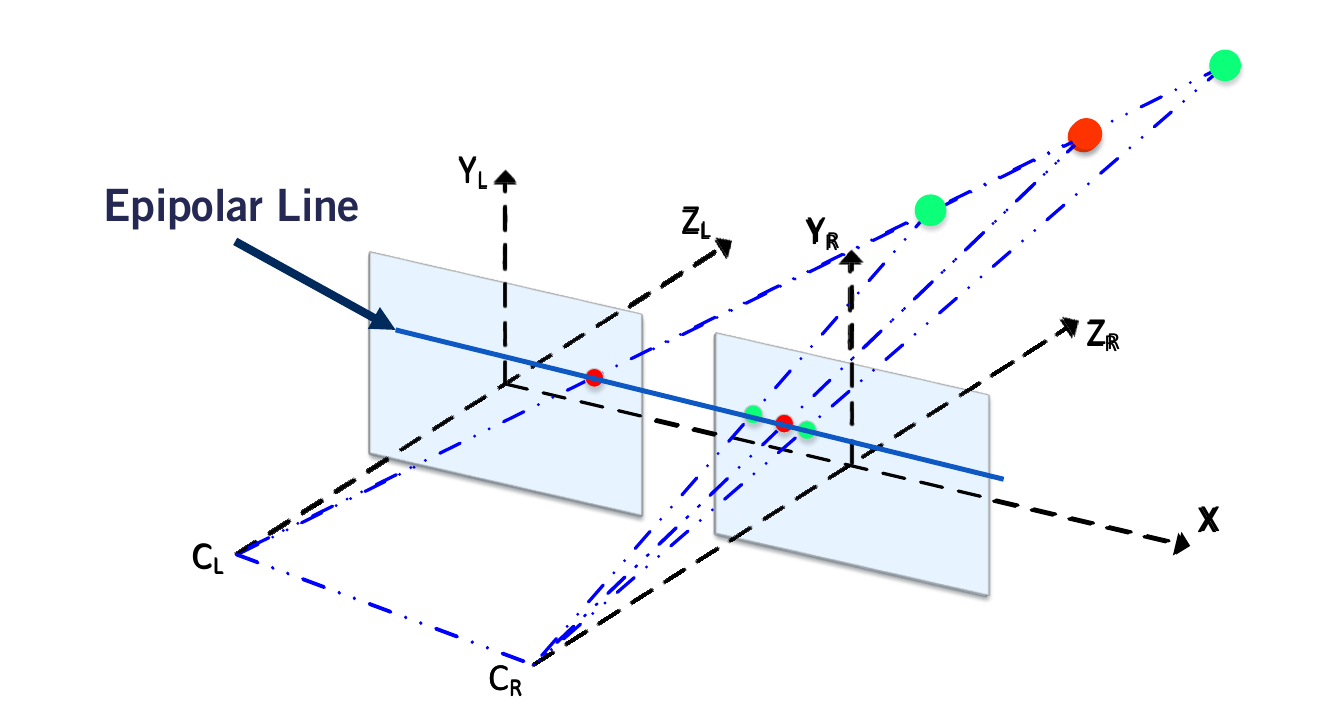
\includegraphics[scale=0.380]{img/visual_perception/epipolar_line.jpeg}
\end{center}
\caption{Epipolar line.}
\label{epipolar_line}
\end{figure}



The epipolar line follows directly from the fixed lateral offset and image plane alignment of the two cameras in a stereo pair. 
We can constrain our correspondence search to be along the epipolar line, reducing the search from 2D to 1D. One thing to note is that
horizontal epipolar lines only occur if the optical axes of the two cameras are parallel. In the case of
non parallel optical axis, the epipolar lines are skewed. In such cases we will
have to result to multiple view geometry rather than the stereo equations we have developed.  

In the case of two calibrated cameras, such as our stereo camera, a skewed epipolar line
is not a huge problem. In fact, we can work the optical axis to be parallel through a process
known as \textbf{stereo rectification}. After rectification we arrive back to our horizontal
epipolar line. We will not go through how to perform rectification
as implementations are available in standard
computer vision packages such as OpenCV and MATLAB. 


\begin{framed}
\begin{remark}{\textbf{Stereo Rectification}}

See the following article on wikipedia about image rectification \url{https://en.wikipedia.org/wiki/Image_rectification}.
Also OpenCV base stereo image calibration \url{https://sourishghosh.com/2016/stereo-calibration-cpp-opencv/}.
\end{remark}
\end{framed}

Let us go over our first basic stereo algorithm.

\begin{enumerate}
\item For each epipolar line take a pixel on this line in the left image
\item Compare these left image pixels to every pixel in the right image on the same epipolar line. 
\item Pick the pixel that has minimum cost. For example, a very simple cost here can be the squared difference in pixel intensities.
\item Compute disparity $d$ by subtracting the right image location from the left one
\end{enumerate}

Stereo matching is a very well-studied problem
in computer vision. Many more complex costs and search regions can be defined, which attempts to improve either computational efficiency
or disparity accuracy. There are a wide range of approaches including both local
and global methods, which differ in the main image region considered when identifying correspondences
and computing disparities. As with most problems in computer vision, the stereo vision algorithms are evaluated 
on a public benchmark. The most famous of which is the Middlebury stereo benchmark, \url{ http://vision.middlebury.edu/stereo/eval3/}. 
If you are interested, many of the top-performing
stereo matching algorithms have results published there
and have code available too. 

\subsection{Summary}

\subsection{Questions}

\subsection{Assignements}

\section{Image Filtering}
\label{image_filtering}

In this section, we will 
be talking about image filtering through cross correlation and
convolution operations. We will also discuss some of the common uses for these operations and relate them to the self-driving task. 

\subsection{Why Do We Need Image Filtering?}
First, let us begin with the motivation on why we
would use image filtering. The image formation process is susceptible to lots of
different noise sources. An example is shown in Figure \ref{camera_man_1}.

\begin{figure}[!htb]
\begin{center}
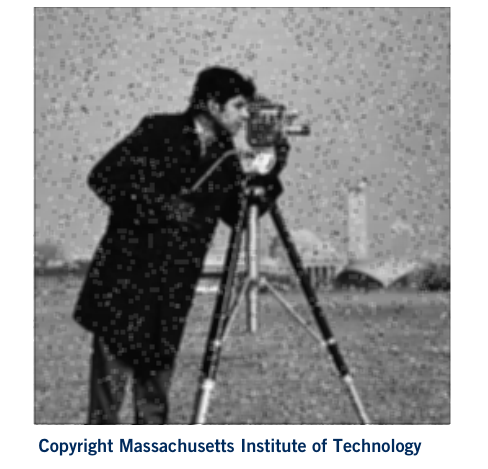
\includegraphics[scale=0.380]{img/visual_perception/camera_man_1.jpeg}
\end{center}
\caption{Example of a noise image.}
\label{camera_man_1}
\end{figure}

This is a very famous photo created at MIT that is used for testing
computer vision algorithms. Now let us add salt and
pepper noise to this image, by randomly turning some of its pixels white
and others black. How can we retrieve a reasonable visual appearance of the original image
from such a noisy one? Image filtering is as simple and efficient method
to eliminate noise. Moreover, depending on the filter, a variety of operations can be performed on images in
an efficient manner. But first, let us see how image filtering helps reduce salt and pepper noise as
a motivating example. 

\subsection{Reduce Image Noise}

If we look at the image array, we noticed that salt and pepper noise usually results in
outlier pixels, low-value pixels in a high-value neighborhood or high-value pixels in a low-value neighborhood, see Figure \ref{camera_man_2}. 

\begin{figure}[!htb]
\begin{center}
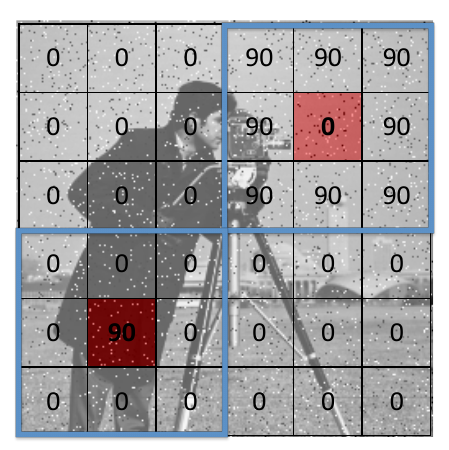
\includegraphics[scale=0.380]{img/visual_perception/camera_man_2.jpeg}
\end{center}
\caption{Schematic of outlier pixels.}
\label{camera_man_2}
\end{figure}

One idea to reduce this noise is to compute the mean of
the whole neighborhood, and replace the outlier pixel
with this mean value. Let us define $G$ as the output
of our filter operation. The equation of the mean can
be described in terms of $k$, $u$ and $v$ as shown in equation.

\begin{equation}
G(u,v) = \frac{1}{(2k+1)^2} \sum_{i=-k}^{k}\sum_{j=-k}^{k} I[u-i, v-j]
\label{simple_filter_equation}
\end{equation} 


Here, $2k+1$ is the filter size. In this case, the size of
our neighborhood which is three leads to a $k$
that is equal to one. $u$ and $v$ are the center pixel
image coordinates. Computing the mean
results in 80 for the top neighborhood and
10 for the bottom one. The final step is to
replace the center pixel of each of those neighborhoods
by the corresponding mean. The application of the so called mean filter results in

\begin{figure}[!htb]
\begin{center}
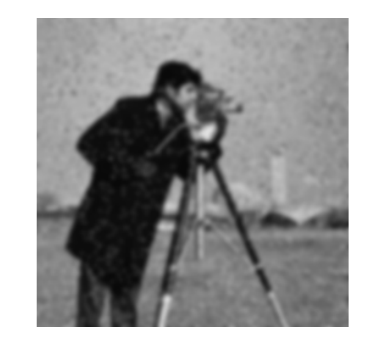
\includegraphics[scale=0.380]{img/visual_perception/camera_man_3.jpeg}
\end{center}
\caption{Camera man image after mean filtering.}
\label{camera_man_3}
\end{figure}

We can see that we have successfully reduced the noise and smooth the image array values in this neighborhood. 
However, it also blurred our image, an inevitable consequence
of these linear filters. This blur can be reduced by tuning the parameters specific to each type of filter.

Equation \ref{simple_filter_equation} can be written as

\begin{equation}
G(u,v) = \frac{1}{(2k+1)^2} \sum_{i=-k}^{k}\sum_{j=-k}^{k} H[i,j]I[u-i, v-j]
\label{simple_filter_equation_2}
\end{equation}

where $\mathbf{H}$ is the weight matrix  called the kernel. We can use $\mathbf{H}$ to add a  weight to every pixel
in the neighborhood.  This generalized form is termed cross-correlation, as it defines a correlation between each pixel and every other pixel in
the neighborhood. For the mean filter defined above, we now represented with the following kernel. A three-by-three matrix filled with the value one-ninth. 

\begin{equation}
\mathbf{H} = \frac{1}{9}\begin{bmatrix}
1 & 1 & 1 \\
1 & 1 & 1 \\
1 & 1 & 1 
\end{bmatrix}
\end{equation}

Another kernel for
noise reduction is the Gaussian kernel, where the center pixel
is weighted more than the neighboring pixels and the weights follow
a Gaussian distribution. 

\begin{equation}
\mathbf{H} = \frac{1}{16}\begin{bmatrix}
1 & 2 & 1 \\
2 & 4 & 2 \\
1 & 2 & 1 
\end{bmatrix}
\end{equation}


Application of a Gaussian kernel in the camera-man image results in Figure \ref{camera_man_4}.  

\begin{figure}[!htb]
\begin{center}
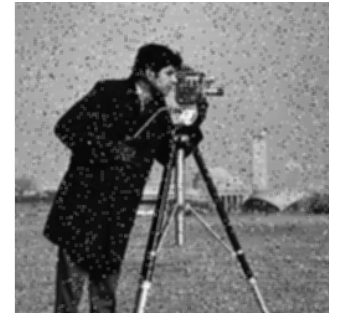
\includegraphics[scale=0.380]{img/visual_perception/camera_man_4.jpeg}
\end{center}
\caption{Camera man image after gaussian filtering.}
\label{camera_man_4}
\end{figure}

\subsection{Convolution Operations}

Now, we will define another useful operation
used for image filtering. A convolution is a cross-correlation, where the filter is
flipped both horizontally and vertically before being
applied to the image. In order to apply the convolution, we take each row of our kernel, flip it and replace it at its corresponding symmetric
position from the middle row. Mathematically, a convolution can be described as
the following equation. Note that we simply manipulated the image coordinates instead
of flipping the kernel. 

What are the advantages of using a convolution over a kernel? Unlike correlation,
convolution is associative, meaning the order of multiplication of
kernels does not matter. We can therefore apply as many consecutive linear kernels
to an image as we want by precomputing
the combined convolution of all the kernels, and then performing
a single convolution of the resulting kernel with the image. As an example, we apply
two linear kernels, $H$ and $F$, by computing $H*F$ and then
applying it to the image. This results in a substantial
reduction in runtime, especially if we need to process images in real-time while
moving in a vehicle. 


\subsection{Applications of Cross-Correlation and Convolution Operations}

Now let's presentsome important applications of cross-correlation and convolution operations. Cross-correlation can be
used for template matching. 

\subsubsection{Template Matching}

Template matching is the problem where we are given a pattern
or a template, and we want to find its location in the image, see \cite{Nazil2013} for an overview. 

\begin{framed}
\begin{remark}{\textbf{Template Matching}}

See the wikipedia entry \url{https://en.wikipedia.org/wiki/Template_matching}. 
See also the OpenCV tutorial on template matching at \url{https://opencv-python-tutroals.readthedocs.io/en/latest/py_tutorials/py_imgproc/py_template_matching/py_template_matching.html}
\end{remark}
\end{framed}

This can be done by finding the location of the highest value of the output
of cross-correlation, between the template and the image. To visualize this better, let's superimpose
the colorized output of cross-correlation on top of our target image. This is shown in Figure \ref{camera_man_5}


\begin{figure}[!htb]
\begin{center}
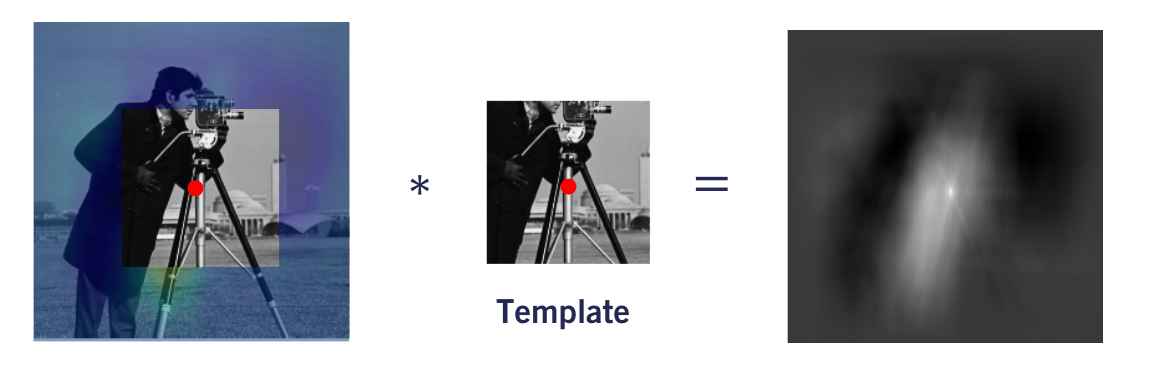
\includegraphics[scale=0.380]{img/visual_perception/camera_man_5.jpeg}
\end{center}
\caption{Template matching.}
\label{camera_man_5}
\end{figure} 


Here red is a high cross-correlation response, while blue is
a very low response. The location of the template
and the image is then the $u, v$ coordinates of the pixel with the highest value from the output of
the cross-correlation. We can check that
our correlation is correct by superimposing
the template on the $u, v$ coordinates we just found. This method can be used as a starting point for
the identification of signs, and even for lean detection, although challenges arise with the approach in practice. 

\subsubsection{Image Gradient Computation}

Another important application that can be performed using convolutions, is image gradient computation. 
This is shown schematically in Figure \ref{camera_man_6}

\begin{figure}[!htb]
\begin{center}
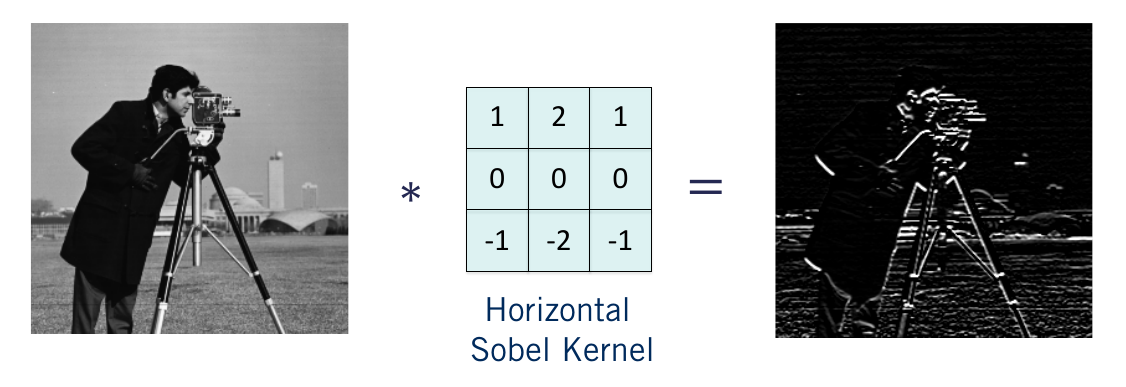
\includegraphics[scale=0.380]{img/visual_perception/camera_man_6.jpeg}
\end{center}
\caption{Schematic of image gradient computation.}
\label{camera_man_6}
\end{figure}

Image gradients can be computed by a convolution with a kernel that performs finite difference. We can rotate our kernel in different orientations
to get vertical, horizontal or even diagonal gradients of an image at a pixel. Image gradients are
extremely useful for the detection of edges and corners, and are used extensively
in self-driving for image feature and object detection, for example. 

\subsection{Summary}

In this section, we discussed how to perform cross-correlation and convolution as well as some of the uses
of these operations. These operations will prove to be very useful later on when we discuss
convolution neural networks. 

\subsection{Questions}

\subsection{Assignements}

\clearpage
%\section{Answers to Questions}
\label{answer_questions}

{\textbf{Answer to questions in section \ref{introduction_self_driving_cars_questions}}}

\begin{enumerate}

\item Which of the following are components of longitudinal control? (Select all that apply)

\begin{itemize}
\item Braking and accelerating are components of longitudinal control. Thus, options 1 and 3 are correct
\end{itemize}

\item Which of the following is not an example of OEDR?

\begin{itemize}
\item Finding routes between locations is a long term planning problem and not OEDR. Hence, option 2 is correct.
\end{itemize}

\item Which of the following tasks would you expect a Level 2 system to perform? (Select all that apply)

\begin{itemize}
\item Options 1 and 3 are correct.
\end{itemize}

\item What is the distinction between Level 3 autonomy and Level 4 autonomy? 

\begin{itemize}
\item Option 4 is correct.  Level 3 systems cannot handle emergencies automatically and as a result require full user alertness.
\end{itemize}

\item What distinguishes Level 5 Autonomy from Level 4?

\begin{itemize}
\item Option 3 is correct. Level 5 systems can operate in any weather condition, on any road type or surface and in any scenario and remain safe.
\end{itemize}

\end{enumerate}

{\textbf{Answer to questions in section \ref{perception_questions}}}

\begin{enumerate}

\item Which of the following tasks are associated with perception? (Select all that apply) 
\begin{itemize}
\item Perception deals with position, motion estimation and object identification. Hence options 1 and 2 are correct.
\end{itemize}

\item Which of the following can be on road objects? (Select all that apply) 

\begin{itemize}
\item Potholes and vehicles are on road objects. So options 1 and 4 are correct.
\end{itemize}

\item Which of the following tasks pose challenges to perception? (Select all that apply) 

\begin{itemize}
\item All four choices pose challenges to perception
\end{itemize}

\item Which of the following sensors are used for ego localization? (Select all that apply) 


\begin{itemize}
\item Global Navigation Satellite System (GNSS) sensor provides position and velocity measurements, and can be used to estimate vehicle position and orientation for localization. An IMU provide acceleration and rotation rate measurements from accelerometers and gyroscopes, and can be used to estimate vehicle orientation and aid in localization in general. Thus, options 1 and four are correct.
\end{itemize}

\item Which of the following objects would be relevant for perception in adaptive cruise control?


\begin{itemize}
\item Adaptive cruise control detects vehicles ahead to control speed and to maintain safe driving distances. So
option 3 is correct. 
\end{itemize}

\end{enumerate}



\bibliographystyle{plain}
\input{references.bbl}
\end{document}
